\title{Maya Soft Body Deformer Plugin Using Shape Matching \\ \large SFX - Tricks of the trade: Project Report}

\author{\begin{tabular}{ccc}
    Isabell Jansson & Ronja Grosz  & Jonathan Bosson \\
    \small isaja187@student.liu.se &\small rongr946@student.liu.se &\small jonbo665@student.liu.se \\
\end{tabular}}
\date{\today}

\documentclass[12pt, twocolumn]{article}
\usepackage{graphicx} % Figures
\usepackage{amsmath}
\usepackage{subcaption}

\newenvironment{myitemize}
{ \begin{itemize}
    \setlength{\itemsep}{0pt}
    \setlength{\parskip}{0pt}
    \setlength{\parsep}{0pt}     }
{ \end{itemize}                  } 


\begin{document}
\twocolumn[
\begin{@twocolumnfalse}
\maketitle

\begin{abstract}

This report follows the approach proposed by M\"uller et al.\cite{shapematching} to simulate soft body deformation using shape matching and examines how it can be implemented into Autodesk Maya as a deformer plugin. The shape matching method does not require storage of any data about neighbouring vertices and is unconditionally stable. Due to its efficiency in terms of memory and computation complexity it is well suited for interactive applications.

\end{abstract}

\end{@twocolumnfalse}
]

\section{Introduction}
    Soft body deformation is a computer graphics method for simulating the deformation of a soft body. 
    There exists many techniques for achieving soft body deformation.
    In this paper we present the method and results from implementing a soft body deformer plugin for the 3D computer graphics software Maya. The implementation is based on the meshless shape matching method proposed by M\"uller et al.~\cite{shapematching}.

\section{Background}
    Soft deformable bodies is a field in computer graphics that focuses on the physical and visual simulation of the motion and characteristics of a soft deformable body.
    Soft deformable bodies are objects whose bodies can change by being deformed without losing its characteristic shape.
    Several different methods have been proposed to simulate the deformation of soft deformable bodies.
    The spring mass model is one of the simpler methods where the soft body is approximated by a set of masses linked by springs.
    The method is popular for simulating the deformation of cloth.
    Two other methods are the finite element method and the energy minimization method.

    The shape matching approach proposed by M\"uller et al.~\cite{shapematching} is a meshless shape matching technique for deformation of soft bodies.
    It is a meshless technique since the object is only represented by a point cloud.
    There is no need for connectivity information between the points since the shape matching keeps the shape of the object.
    This is done by driving the deformed points towards the position of the points of the original shape, see figure~\ref{fig:def}.
    
    \begin{figure}
    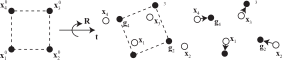
\includegraphics[width=\linewidth]{img/deformation2.png}
    \caption{The shape matching process where the original shape $\mathbf{x}^0_i$ is matched to the deformed shape $\mathbf{x}_i$ and pulled towards the goal shape $\mathbf{g}_i$. Image source:~\cite{shapematching}.}
    \label{fig:def}
    \end{figure}
    
\section{Shape matching implementation}
    The soft body is represented by a point cloud, where each particle has a mass $m_i$, an initial position $\mathbf{x}_i^0$ representing the shape of the object and a deformed position $\mathbf{x}_i$.
    The soft body is affected by external forces such as gravity, collision impulse and friction impulse caused by a collision with an object.
    The external forces $f_{ext} = F_g + J_c + J_f$ is what causes the deformation of the soft body.
    The new velocities and positions for the particles are calculated using the external forces and Euler integration.
    The collision impulse $J_c$ is calculated through Equation~\ref{eq:col} where $\epsilon$ is the elasticity of the soft body, $n$ is the contact normal and $\Delta{v}$ is the velocity difference between the soft body and the static object it collides with.
    The friction impulse is calculated through Equation~\ref{eq:fric}, where $f$ is the friction.

    \begin{equation} \label{eq:col}
        J_c = -(1 + \epsilon)(n(n\cdot{\Delta{v}}))m_i
    \end{equation}

    \begin{equation} \label{eq:fric}
        J_f = -f(\Delta{v} - n(n\cdot{\Delta{v}})m_i
    \end{equation}

    The shape matching is made by finding a goal position $g_i$ for every particle.
    The goal position is used to find the new velocities and positions for the particles for each time step, driving the soft body to take its original shape at $\mathbf{x}^0$.
    The new velocities and positions are calculated through Euler integration where $\alpha$ is the bounciness and stiffness of the soft body and $h$ is the time step, see Equation~\ref{eq:vel} and~\ref{eq:pos}.

    \begin{equation} \label{eq:vel}
        \mathbf{v}_i(t + h) = \mathbf{v}_i(t) + \alpha{\frac{\mathbf{g}_i(t) - \mathbf{x}_i(t)}{h}} + hf_{ext}(t)/m_i
    \end{equation}

    \begin{equation} \label{eq:pos}
        \mathbf{x}_i(t + h) = \mathbf{x}_i(t) + h\mathbf{v}_i(t + h) 
    \end{equation}

    The goal position is found through the rotation matrix $\mathbf{R}$, the initial position $\mathbf{x}^0_i$, the center of mass for the initial position $\mathbf{x}^0_{cm}$ and the center of mass for the current deformed shape $\mathbf{x}_{cm}$, see Equation~\ref{eq:goal}.
   
    \begin{equation}\label{eq:goal}
        \mathbf{g}_i = \mathbf{R}(\mathbf{x}^0_i - \mathbf{x}^0_{cm}) + \mathbf{x}_{cm}
    \end{equation}

    The rotation matrix is approximated through the linear transformation $\mathbf{A}$, see Equation~\ref{eq:A}.
    The linear transformation is composed of the relative locations $\mathbf{q}_i = \mathbf{x}^0_i - \mathbf{x}^0_{cm}$ and $\mathbf{p}_i = \mathbf{x}_i - \mathbf{x}_{cm}$, see Equation~\ref{eq:com1} and~\ref{eq:com2}.
    The rotation $\mathbf{R}$ is the rotational part of $\mathbf{A}_{pq}$ which is found through singular value decomposition.

    \begin{equation} \label{eq:A}
        \mathbf{A} = (\sum_i{m_i\mathbf{p}_i\mathbf{q}_i^{\mathbf{T}}})
        (\sum_i{m_i\mathbf{q}_i\mathbf{q}_i^{\mathbf{T}}})^{-1} 
        = \mathbf{A}_{pq}\mathbf{A}_{qq}
    \end{equation}

    \begin{equation} \label{eq:com1}
        \mathbf{x}^0_{cm} = \frac{\sum_i{m_i\mathbf{x}_i^0}}{\sum_i{m_i}}
    \end{equation}

    \begin{equation} \label{eq:com2}
        \mathbf{x}_{cm} = \frac{\sum_i{m_i\mathbf{x}_i}}{\sum_i{m_i}}
    \end{equation}

    \paragraph{Rigid deformation}\mbox{}\\[5px]
    For a rigid deformation $\alpha$ is set to one, moving the points to the goal position $\mathbf{g}_i$ exactly for each time step.
    The goal position represents a rotated and translated version of the initial shape.

    \paragraph{Linear deformation}\mbox{}\\[5px]
    For linear deformation, the linear transformation $\mathbf{A}$ in combination with the rotation matrix $\mathbf{R}$ according to Equation~\ref{eq:T} is used instead of the rotation matrix to calculate the goal position, see Equation~\ref{eq:goal}.
    The linear deformation $\mathbf{A}$ is divided by $\sqrt[3]{det(\mathbf{A})}$ to keep the volume conserved.

    \begin{equation} \label{eq:T}
        \beta\mathbf{A} + (1 - \beta)\mathbf{R}
    \end{equation}

    \paragraph{Quadratic deformation}\mbox{}\\[5px]
    To extend the motion to twisting and bending a quadratic transformation is applied.
    $\mathbf{q}$ is extended to $\mathbf{\tilde{q}} = [\mathbf{q}_x, \mathbf{q}_y, \mathbf{q}_z, \mathbf{q}_x^2, \mathbf{q}_y^2, \mathbf{q}_z^2, \mathbf{q}_x\mathbf{q}_y, \mathbf{q}_y\mathbf{q}_z, \mathbf{q}_z\mathbf{q}_x]^\mathbf{T}$.
    With the new $\mathbf{\tilde{q}}$, a new linear transformation $\mathbf{\tilde{A}}$ can be calculated the same way as Equation~\ref{eq:A}.
    To keep the volume, $\mathbf{\tilde{A}}$ is divided by $\sqrt[9]{det(\mathbf{\tilde{A}})}$.
    Together with the rotation matrix $\mathbf{\tilde{R}} = [\mathbf{R~0~0}]$, the goal position is calculated according to Equation~\ref{eq:newGoal}.

    \begin{equation} \label{eq:newGoal}
        \mathbf{g}_i = (\beta\mathbf{\tilde{A}} + (1 - \beta)\mathbf{\tilde{R}})\mathbf{\tilde{q}}
    \end{equation}
    

\section{Maya Implementation}

The plugin is built upon the deformer node, $MPxDeformerNode$, in Mayas C++ API which can control the position of all vertices of an object with the deformer loaded. By copying the vertice positions as individual particles in a custom particle system in the plugin more control gained. A bigger freedom is also gained which allows the use of high quality linear algebra libraries for efficient and complex calculations. 

As seen in \ref{fig:gui}, the deformation of a shape can be controlled by changing the following parameters:

\begin{myitemize} 
  \item Gravity Magnitude and Direction 
  \item Mass, $m$
  \item Stiffness, $\alpha_s$ - $[0,1]$ variable controlling how much deformation is allowed
  \item Bounciness, $\alpha_f$ - $[0,1]$ variable controlling the strength of the overshoot
  \item Friction, $f$
  \item Deformation, $\beta$ - $[0,1]$ variable controlling the strength of the deformation
  \item Elasticity, $\epsilon$
  \item Mode (Rigid, Linear or Quadratic) - Controls the kind of desired deformation 
  \item Initial Velocity 
\end{myitemize}

The local time variable is connected to the global time so that the deformation will update when the timeline changes. The plugin stores the value of the last time step so the simulation behaves correctly regardless of how the global time is changed. Further variables can be linked with other parameters in maya such as the gravity magnitude and direction can take their values from a gravity field.

 \begin{figure}[t]
    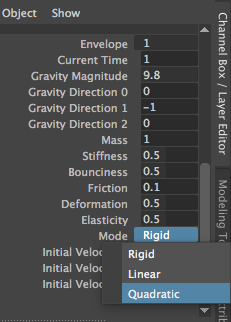
\includegraphics[width=\linewidth]{img/gui.png}
    \caption{The user interface in Maya which is used to modify the deformation.}
    \label{fig:gui}
    \end{figure}

\section{Conclusion}

The deformer node plugin can handle rigid as well as soft body (linear and quadratic) deformations with a low computation cost. Figure \ref{fig:maya} illustrates the deformation that happens when a sphere collides with the ground plane. After impact, in \ref{fig:sfig2}, will the mesh reform into a egg-like shape to later settle down as the original sphere.

\begin{figure}
\begin{subfigure}{.3\textwidth}
  \centering
  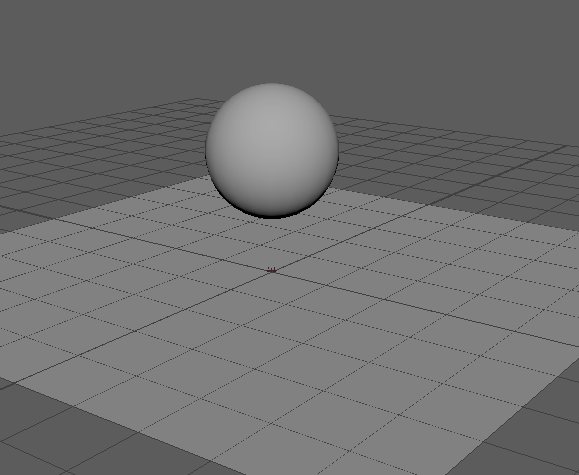
\includegraphics[width=0.9\linewidth]{img/def1.png}
  \caption{}
  \label{fig:sfig1}
\end{subfigure}%
\begin{subfigure}{.3\textwidth}
  \centering
  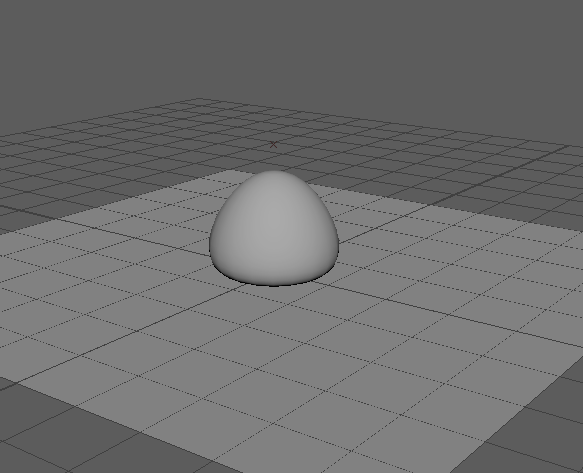
\includegraphics[width=0.9\linewidth]{img/def2.png}
  \caption{}
  \label{fig:sfig2}
\end{subfigure}
\caption{A quadratic deformation of a sphere using the plugin.}
\label{fig:maya}
\end{figure}

%Picture of IBL rendered deformation, comment on that in results.


\section{Discussion and Future Work}

The shape matching method can be useful in rigid and moderately soft body deformations even though the algorithm is not physically grounded. It can model twists and bends well but struggles with stability with large deformations. If the parameters $bounciness$ or $deformation$ is set too high the deformed positions cannot adequately be translated to their goal position, which causes the shape to be flattened upon impact with the ground plane. Proper parameter management is therefore required.

Another possible extension to the plugin could be to implement support of object to object collision. Current solution only handles collision with the ground plane by naively checking if the a particles y-value is below the y-value of the plane to then respectively updates the forces.

\bibliographystyle{ieeetr}
\pagebreak
\bibliography{./refs}

\end{document}
